% !TEX root = ../Dissertation-vLautz.tex

\chapter{Introduction}

\label{ch:Introduction}
In this particularly hot summer it is not beyond imagination that you choose to buy a watermelon from a small stand on the way home. Of course, you wish to buy not any watermelon, but a ripe and juicy one. According to humourist literature \parencite["fixating the melon's secret",][]{Kishon1975} the procedure of selecting a ripe and juicy melon consists of looking, feeling, smelling, and listening for a hollow sound and then comparing these features to another watermelon. Moreover, if the quality of tested watermelons doesn’t suit you, you go to the next stand and try the ones there. This example encompasses several features of typical decision-making tasks used in neuroscience. To find just the right watermelon you need to \textit{perceive} the colour, texture, smell, and sound. Then, you must keep this information for a short while in \textit{memory} before testing the subsequent watermelon. Finally, you are tasked with judging which one was better: \textit{making a decision}. Neuroscientists use such tasks in simple form to have control about the mental steps necessary to correctly solve this problem. For example, they would typically let participants only see the melons and let them decide between two, a challenge called ‘sequential comparison task’. Or an experimenter would give participants the job of testing watermelons from multiple stands and deciding whether they were of good or poor quality. In this case, a person would need to \textit{sequentially sample} watermelons up until she is confident that the particular stand sells good- or poor-quality fruit. In contrast with the study of psychophysics, which tests only the behaviour of participants, neuroscientists typically also record signals from the brain during such tasks and try to determine the neural basis of each mental step (e.g., \textit{perceiving, memory, making a decision}). 

In the present thesis, I will introduce how neuroscientists study such decisions in humans and other species. I will describe major lines of research investigating the neural substrates of the outlined mental steps using two well-studied experimental paradigms that fit to the aforementioned watermelon selection: sequential comparison and sequential sampling tasks. Then I will present my contribution to this field of research in the form of three studies that provide new insights into human working memory and decision making with magneto- and encephalography (M/EEG). Subsequently, I will link my findings to the larger context of current research and point to future avenues. 

\section{Researching perceptual decision making}
The study of human decisions has a long history reaching back to ancient Greece \parencite{Aristotle1987,Epicurus1940}. Whereas Greek philosophers argued for a nonmaterial soul determining all behaviour, the Enlightenment challenged this view and in particular \textcite{Descartes1649} advocated a dualist approach, where simple motor behaviours could be explained by actions of the material body \parencite{Descartes1664,Descartes1988}. In the 19th century Gustav Fechner went one step further and used empirical methods%\footnote{For a wonderful introduction into empirical methods see: \url{www.hpmor.com}} \parencite{Bacon1620}
 to unite behavioural measures with subjective, individual perception \parencite{Fechner1860}. Similar to my introductory task with watermelons, Fechner tasked volunteers to lift two weights in succession and questioned them which was heavier, a sequential comparison task. This simple task provides a powerful tool to study human behaviour, because it allows to control an objective stimulus variable – the weight – and observe subjective perceptual differences between stimuli. Using this approach, Fechner was able to describe a logarithmic mapping between the physical magnitude of a stimulus and the extend of sensation it produces, the Weber-Fechner law that gave first insights into possible constraints of how information is processed by humans. Psychophysics, as Fechner called his mathematical descriptions of human psychology, has been aided in the study of the human brain by the invention of signal detection theory (SDT). Originally used to classify the detection of weak signals, the SDT proposes that an observer can respond to a stimulus in four ways: detect (hit), not detect (miss), detect the absence (correct reject), erroneously detect (false alarm). The advantage over conventional methods of only analysing hits and misses is that the SDT assumes an internal measurement of the stimulus feature that is proportional to the actual feature but includes noise. Therefore, also correct rejections and false alarms provide evidence for the internal measurement. The decision process for a given stimulus can be modelled as taking a sample of two overlapping noisy (gaussian) distributions and applying a simple criterion. Most notably for the present thesis, we can take multiple samples from a stimulus over time and get ever-improving estimates of whether the stimulus belongs in one or the other part of the two overlapping distributions. Conceptually, this can be seen as accumulating evidence before applying a criterion. In the context of decision making studies, the internal measurement that we take for a stimulus is often referred to as a decision variable (DV). This DV has been linked closely to neuroscience, because an area involved in decision making should exhibit neural activity that correlates with the DV throughout an experimental task \parencite{Tanner1954,Gold2007}. Experiments therefore are usually optimized to separate the mental steps involved in the decision processes in time or include only one stimulus feature that has to be detected by accumulating evidence. In the following, I will introduce results from two of the most common experiments operationalized to investigate the neural activity underlying decision making. 

\section{Sequential Comparison Tasks}
Sequential comparison tasks, as Fechner used, are still an important tool to study psychophysics and have had a great impact onto neuroscience when used in conjunction with measurements of neural responses from the brain of primates and rodents. \textcite{Mountcastle1969} were first to train monkeys in a vibrotactile version of this task, termed sequential frequency comparison (SFC) task, and recorded neural data \parencite{Mountcastle1967,Mountcastle1990}.
In this setup (figure~\ref{fig:SFCtask}), a subject is presented with two vibrotactile frequencies in the flutter range (~5-50 Hz), namely frequency 1 ($f1$) and frequency 2 ($f2$).
\begin{figure}[t]
\centering
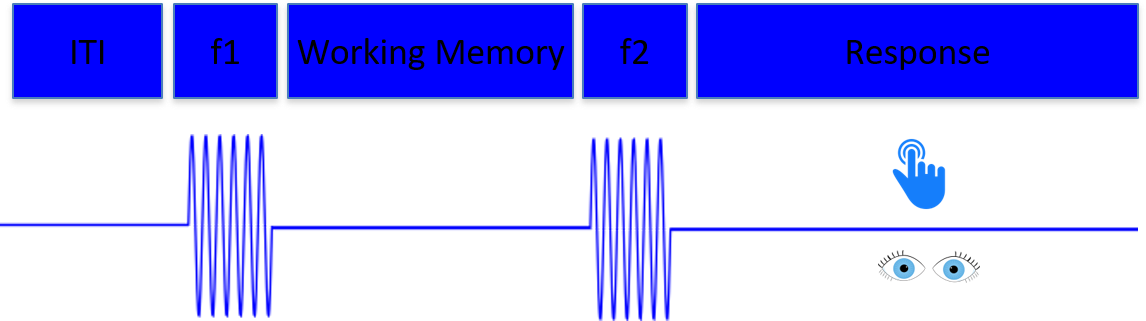
\includegraphics[width=1\textwidth]{figures/SFC_task.png}
\caption{Sequential frequency comparison (SFC) task. Two vibrotactile frequencies are presented to the index finger in succession, $f1$ and $f2$. The task is to decide whether $f2$ is larger than $f1$ or vice-versa. Between $f1$ and $f2$ is a working memory interval in which the frequency of the first stimulus has to be retained. After perception of $f2$, responses are made, typically via button press or saccade.}
\label{fig:SFCtask}
\end{figure}
The task is to decide whether the second ($f2$) frequency is higher or lower than the first ($f1$). To solve this challenge the subject must sequentially go through cognitive processes that are classically split into four parts. First, $f1$ is perceived. Second, $f1$ is being kept in memory, while the subject waits for the subsequent stimulus. Third, $f1$ is compared with the perception of $f2$, thereby forming a decision.  Fourth, the subject reports the choice, usually by pressing a button or enacting a saccade to a choice-specific visual target.
\subsection{Sequential Comparison Tasks: Perception}
Perception of the first stimulus drives quickly adapting (QA) neurons in Brodmann areas 1 and 3b of the contralateral primary somatosensory cortex (SI). These neurons receive afferent signals from mechanoreceptors in the skin, which are routed via the Thalamus and are closely interconnected \parencite{Merzenich1969,Mountcastle1967,Talbot1968}. The majority of monkey SI neurons align their spiking activity to the periodicity of the stimulus, which can also be observed in human M/EEG as steady-state evoked potentials/fields (SSEP/F) \parencite{Mountcastle1990,Nangini2006,Tobimatsu1999}. Moreover, a portion of S1 neurons increase their firing rate monotonically with increasing vibrotactile frequency \parencite{Hernandez2010,Hernandez2000,Lemus2010,Luna2005,Salinas2000}. Notably, only those QA neurons that modulate their firing rates by the vibrotactile frequency showed differential patterns in error trials, indicating that the brain uses these neurons to inform behaviour \parencite{Salinas2000}. Therefore, it is well-established that the firing rates and the rhythmic signal observed with M/EEG represent the encoding of sensory evidence on which later decisions are based. Interestingly, the firing rate predicts the monkeys’ behaviour better than the periodicity of the neural responses and while periodicity is high in SI, it is almost absent in SII, speaking against a communication mechanism through periodic firing as would be predicted from SSEPs \parencite{Hernandez2000,Luna2005,Salinas2000}. An alternative possibility is that QA neurons encode stimuli by the number of discrete bursts of spikes instead of single spikes. Such a coding scheme has been observed in visual tasks and has been suggested to efficiently encode stimulus features  \parencite{Kepecs2003,Kepecs2002,Krahe2004,Reinagel1999,Romo2013}. Notably, because other relevant monkey work has focused on bursts \parencite[e.g.,][]{Lundqvist2016}, the stimulation times extend beyond the time of a burst in these vibrotactile studies (always 500ms) and therefore a code based on spikes is indistinguishable to one based upon bursts \parencite{Romo2013}. However, it remains unclear if bursting covaries with behavioural performance on a trial-by-trial level as observed for spikes \parencite{Luna2005}. Regardless whether bursting or spiking underlies an encoding by rate, such a code could be positively or negatively correlated in upstream areas, as is observed throughout the sensorimotor hierarchy in this task including SII, prefrontal and motor cortices \parencite{Hernandez2010,Salinas2000}.

\subsection{Sequential Comparison Tasks: Working Memory}
Such a dual rate code, with populations either increasing or decreasing with stimulus frequencies, was also observed in the absence of stimulation: during the short retention interval between $f1$ and $f2$. In particular, \textcite{Romo1999} recorded from the inferior convexity of the prefrontal cortex and identified neurons whose firing rate changed monotonically with the vibrotactile frequency held in working memory (WM). Visual WM tasks have long associated sustained prefrontal firing with WM \parencite{Funahashi1989,Fuster1971,Goldman-Rakic1995}, however, this study demonstrates that the contents of WM can directly map onto firing rate changes in single neurons. Further analyses indicate that the representation of stimulus information by population dynamics of prefrontal neurons degrades after stimulus presentation, but re-emerges with different tunings towards the end of the working memory delay \parencite{Barak2010}. This is particularly interesting, because it challenges the view that WM is encoded in sustained firing throughout delay periods, with biophysically plausible alternatives both in rhythmicity \parencite{Fiebig2017,Lundqvist2018a,Lundqvist2016} and synaptic changes \parencite{Mongillo2008,Stokes2015}. This current high-level debate \parencite[for either side, see:][]{Constantinidis2018,Lundqvist2018} is so interesting for vibrotactile SFC studies, because firing rates directly represent the contents of WM, not overall changes. Recent evidence, however, suggests that both single neurons and populations may be responsible for WM in this task. \textcite{Haegens2017} recorded local field potentials (LFPs), which reflect local neuronal ensembles, and single neurons from monkey premotor cortex during a multimodal version of the SFC task. They found a modulation of LFP beta oscillations reflecting the stimulus features during WM. In addition, premotor spike-field coherence with the beta band was also related to the stimulus features, indicating a tuning of firing rate to this rhythm. These findings suggest that both population-related beta modulations and the closely affiliated spike activity both encode the contents of WM.
This close coupling of beta oscillations with spiking activity underlying tactile WM has also been suspected from a series of EEG studies. \textcite{Spitzer2010} gave human volunteers a similar SFC task and found a parametric modulation of the beta band in the right inferior frontal gyrus (IFG), suggesting that both monkey and human prefrontal cortices (PFC) exhibit content-specific activity during WM. In a follow-up study, \textcite{Spitzer2011} demonstrated that this prefrontal activity was independent of encoding processes, by retro-cueing to one of two presented vibrotactile stimuli. Furthermore, \textcite{Spitzer2012} hypothesized that this parametric encoding of abstract magnitudes was supramodal. In addition to the tactile task, they implemented a sequential visual flicker and a sequential acoustic flutter comparison task. Across all these modalities, prefrontal beta power monotonically encoded the frequency information of the stimulus. However, this parametric code consists of a monotonic increase in beta power with the vibrotactile stimulus held in working memory and did not exhibit the negative component of a dual code as had been observed in monkey PFC \parencite{Romo1999}. Because the precise link between the large-scale signals recorded with EEG and single neuron firing rates are poorly understood, it remains unclear whether the difference in power reflects a population imbalance of the dual code observed in monkeys, where about 60\% of modulated neurons reflected a monotonic increase \parencite{Romo1999,Spitzer2010}. This is of particular note, because working memory has been associated with sustained firing rates in the PFC \parencite{Funahashi1989,Fuster1971,Goldman-Rakic1995,Pasternak2005} and gamma, not beta, appears to be closely related to neural firing rates even when recorded with surface EEG \parencite{Whittingstall2009}. However, increases in gamma activity during working memory do not necessarily reflect sustained firing rates, but a more dynamic system of neural firing patterns \parencite{Cromer2010,Durstewitz2006,Shafi2007,Stokes2013}. Indeed, recent monkey recordings revealed a pattern of brief gamma bursts accompanying encoding and re-activation of stimulus information while beta bursts reflected a default state of maintenance that was interrupted by gamma \parencite{Lundqvist2016}. Notably, it is quite possible that such short gamma bursts have been averaged out of datasets by summation over multiple trials to increase the signal to noise ratio in previous human recordings \parencite{Stokes2016}. Furthermore, during EEG recordings the skull acts as a low-pass filter \parencite{Pfurtscheller1975}, making it difficult to pick up on gamma oscillations. The only MEG study investigating gamma in an SFC task, found overall gamma increases in SI, SII and frontal cortices during working memory, but did not investigate the parametric encoding of stimulus features \parencite{Haegens2010}. Therefore, it remains an open question how the parametric beta band modulations observed by Spitzer and colleagues are associated with dynamic changes in gamma frequencies. 
\subsection{Sequential Comparison Tasks: Decision Making}
The next part of the SFC task, comparing $f1$ and $f2$ to form a decision is associated with neural firing in premotor cortices (PMC) that are modulated by subtracting $f1$ from $f2$ \parencite{Hernandez2010,Hernandez2002,Jun2010,Romo2004}, which has also been observed in SII \parencite{Romo2002}. Notably, the decisions were indicated by button press and therefore likely associated with PMC rather than with FEF when responses are indicated with saccades \parencite[see also][]{Gold2007}. Underlining this function, the PMC firing rates were modulated reversely during incorrect trials, indicating that they followed the monkey’s choice rather than the physical attributes of the stimuli \parencite{Hernandez2002,Romo2004}. Most interestingly, because the retention of vibrotactile stimuli was associated with beta power in humans \parencite{Spitzer2010}, \textcite{Haegens2011} recorded local field potentials (LFPs) from monkey PMC and found that beta band power reflected the difference between $f2$ and $f1$. Importantly, when monkeys were instructed to respond independent of the task, neural firing and beta LFPs were not modulated by the decision process in PMC \parencite[see also][]{Haegens2017}. These findings in monkeys correspond well to recent EEG studies extending a role of the beta band for decision making to humans during this task \parencite{Herding2016,Herding2017}. Agreeing with \textcite{Haegens2011}, \textcite{Herding2016} demonstrated that beta band power in premotor areas was modulated by participants’ choices, always with the decision outcome $f2>f1$ resulting in a larger beta response than the outcome $f2<f1$. These same findings were replicated for saccade responses, and in line with an intentional framework for decision making \parencite{Shadlen2008}, the beta modulation was source localized to the FEF instead of PMC \parencite{Herding2017}. Moreover, these studies used Bayesian modelling of participants’ behaviour to estimate the subjective contribution of beta to choices, revealing both a clear pattern of beta invariant to the response mapping (index/middle finger) and a scaling by choice even when trials were incorrect. Yet, it remains unclear whether this choice-related beta band effect in the EEG extends beyond somatosensory processing, which has been associated closely with this frequency band \parencite{Pfurtscheller1981}. 
Building upon this finding of choice-related beta modulation, \textcite{Ludwig2018} added a response delay, in which the response mapping was not provided to this task. With this slight change in setup, they found an almost identical beta band effect in the posterior parietal cortex (PPC), but not in premotor areas. This indicates that premotor areas are only directly involved in the decision process when the decision outcome is known. The PPC on the other hand appears to fulfil an effector-unspecific role and might have a more general role in the decision process. This is particularly interesting, because another parietal signal, the classic P300 \parencite{Chapman1964,Sutton1965}, has long been associated with decision making \parencite{Donchin1967,Rohrbaugh1974}. More so, the P300, recently also termed centro-parietal positivity (CPP - more on it later), has been theorized not to reflect a unitary neural event after stimulus onset, but a dynamically changing neural signature of making a decision over time \parencite{Twomey2015}.  Thus, the question remains how the choice related beta band effect in SFC tasks relates to decision signals in other paradigms, specifically the CPP and beta-gamma modulations observed with MEG in accumulation of evidence tasks \parencite{Donner2009,Donner2007,Kelly2013,Kelly2015,OConnell2012,Twomey2016,Twomey2015,Philiastides2014}
\section{Accumulation of Evidence Tasks}
The other line of research I want to introduce builds also on Fechner’s work on psychophysics, and in particular is the result of his legacy in mathematical psychology that drove ever-improving accounts of choice behaviour throughout the 20th century. This led to the development of signal detection theory, which as previously mentioned, has the advantage of taking into account noise behaviour and the structure of incorrect trials \parencite{Tanner1954}. Neuroscientific experiments have used this theory to model perceptual decision making as a process of sequential sampling that results in an accumulation of evidence for a decision. Underlying this model is the idea that a decision variable (DV) represents the set of all evidence for a decision and for binary choices modern models posit a single mechanism that accumulates evidence over time for one choice over another \parencite{Shadlen2013}. For example, in our introductory example when we strive to find a good watermelon stand, we would sample melons from one stand sequentially, until we are sure the stand sells fruit of high or low quality. Every time we try a fruit, we would get a piece of evidence in favour of one possible choice, which over time accumulates to inform a decision – typically modelled as crossing an absolute bound. The neuroscientific hypothesis is that one decision variable tracks the current state of such evidence accumulation and that we can observe such a variable in the brain. 
To track this neural correlate of perceptual decision making, neuroscientists have used predominantly one decision making task: the random-dot motion (RDM) direction discrimination. In the RDM task (figure \ref{fig:RDMtask}) participants are shown dots on a monitor that move around. A portion of these dots move coherently in the same direction and the challenge is to detect this movement. Because the number of dots moving coherently is typically low and movement can only be spotted through a change over time, the perceptual challenge is usually difficult, and it can take between a few hundred milliseconds to seconds to detect the motion. Moreover, because the dots typically move randomly, it is possible to perceive a wrong direction.

\begin{figure}[t]
\centering
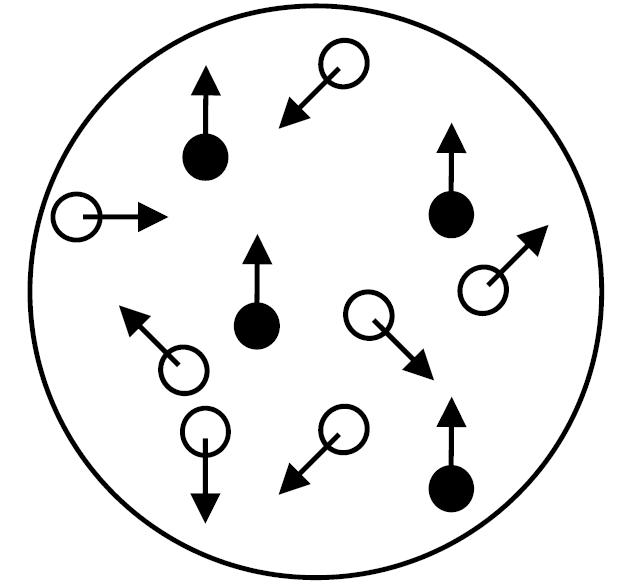
\includegraphics[width=.3\textwidth]{figures/RDM_task.png}
\caption{Example of random-dot motion kinematogram. The white dots represent the dots moving randomly, the black ones the coherently moving dots. The task is usually to detect coherent motion, varying the number of coherently moving dots determines the difficulty and time needed to perform the judgement.}
\label{fig:RDMtask}
\end{figure}

This task is particularly powerful for psychophysics, because it requires no distinct working memory process and it lends itself well to be modelled as an accumulation-to-bound process \parencite{OConnell2018}. In such models it is assumed that subjects continuously sample from the dot-motion stimulus, perceive the motion direction of individual dots and accumulate evidence for one direction over time. When participants have a level of confidence in the direction, the decision bound is crossed and the decision communicated. This is usually done in monkey experiments by eye movements. The model can be further simplified by having the subjects decide between two opposite directions that are known in advance, thus becoming a binary accumulation process. Notably, because choices are typically indicated by performing a saccade to one of two targets associated with the choices, the decision process can be treated as a process of movement selection. Therefore, beyond motion sensitive neurons in MT/V5, recordings are primarily carried out in those areas associated with motor preparation and eye-movement execution, resulting in neural correlates of a decision variable in the superior colliculus (SC), frontal eye fields (FEF), lateral intraparietal area (LIP) and the dorsolateral prefrontal cortex (DLPFC) \parencite[for review see][]{Gold2007}. 

\subsection{Accumulation of Evidence Tasks with Nonhuman Primates}
Employing the RDM task while recording from macaques, \textcite{Britten1992} were able to link a small set of middle temporal visual area (MT/V5) neurons to concurrent choice behaviour. Even when the coherence was at 0\% and all dots were moving randomly, MT firing rates predicted choices significantly \parencite{Britten1996}. Motion sensitive neurons in area MT are well-known to respond strongly to visual stimuli moving in a particular direction, exhibiting tuning to stimuli moving through their receptive fields \parencite{Baker1981,VanEssen1981,Zeki1980,Zeki1974}. Using this knowledge of systematic motion direction organization in MT, microstimulation has been used to successively activate motion direction specific systems, thereby demonstrating a causal relationship of MT neurons for task performance \parencite{Ditterich2003,Salzman1990,Salzman1992}. Most interestingly, when using a version of the RDM task with the opportunity to respond as soon as possible, MT microstimulation influences both choice and RTs in the stimulated neurons’ preferred motion direction. In turn, when MT neurons are deactivated, the decision making process is impaired, likely because the sensory encoding is interrupted \parencite{Katz2016}. On a functional level these findings indicate that MT processes the motion information and thus provides the sensory evidence on which decisions are formed.

To find out the neural substrates of a decision variable, a large body of monkey recordings targeted the FEF, because it is well-connected to visual areas, and known to encode the saccade processing required to respond in the RDM paradigm \parencite{Felleman1991,Hanes1996,Schall1995,Schall1995a,Thompson1996,VanEssen1992}. Moreover, suprathreshold electrical stimulation evokes saccades while subthreshold stimulation elicits changes to saccade selection and spatial attention \parencite{Burman1997,Moore2001,Moore2003,Robinson1969}. \textcite{Gold2000} interrupted motion viewing during the evidence accumulation process while monkeys viewed the RDM stimuli. Then they immediately applied a short electrical current to the FEF, which resulted in a saccade whose direction and amplitude was influenced by the current state of the decision process, reflecting the evolution of a decision variable \parencite{Gold2000,Gold2003}. However, while the FEF is clearly involved in the decision process, it appears that only a small part of FEF neurons track the DV, while others encode stimulus properties during and after the decision, possibly to evaluate the outcome \parencite{Ding2012}. Together, these studies indicate that the FEF is related to action-performance in RDM tasks with saccade responses, but also encodes stimulus and outcome related information.

Besides the more perceptual aspects of MT and the action-related activity in FEF, the lateral intraparietal area (LIP) has been extensively studied in RT-dependent versions of the RDM task. LIP has been focused on, because anatomically it receives inputs from MT and outputs to the FEF \parencite{Andersen1992,Blatt1990,Lewis2000}. In particular, the LIP is tightly coupled to areas involved in eye movement control \parencite{Andersen1990}. FEF neurons fire when a saccade is planned into their receptive fields \parencite{Andersen1987} and its neurons fire persistently when an animal withholds a saccade to a target \parencite{Barash1991,Gnadt1988}. Thus, LIP function appeared to be between perceptual processing and eye-movement execution, responsible for sensorimotor integration mediated by cognitive control \parencite[for review,][]{Andersen2002}. Therefore, it was unsurprising when \textcite{Shadlen1996,Shadlen2001} demonstrated that activity in LIP neurons, whose receptive fields were aligned with visual targets in the RDM task, increased before saccades to these targets were executed. Surprisingly however, single neuron activity was modulated by the presentation of dot-motion and correlated with RDM coherency. That is, activity reflected the difficulty of individual RDM patches by faster increases of firing rates in easy trials, indicating that LIP neurons tracked the evolution of the decision process. Most interestingly, LIP firing rates accumulated to a fixed threshold at the time of response independent of trial difficulty, fitting to drift-diffusion models of decision processing \parencite{Roitman2002a,Shadlen1996,Shadlen2001}. Contrary to MT however, LIP microstimulation appears to only slightly affect choice and RT \parencite{Hanks2006}. Moreover, when short motion pertubations were added to the RDM kinematogram, RT and choices were modulated by these over a sustained period of time \parencite{Huk2005}. Together, these findings indicate that LIP neurons reflect the integration of decision information over time and microstimulaton pertubations drive the encoded decision variable with respect to a decision bound. 
Most relevant to the present thesis (task design study 1 \& 3), when responses could not be immediately taken and monkeys had to map targets to a spatially undetermined color-code, LIP neurons still represented the DV even though no specific saccade planning was possible \parencite{Bennur2011}. This indicates that LIP function includes tracking the evolving DV independent of a specific motor response. However, a recent study using causal de-activation of LIP neurons during decision formation suggests that LIP neurons may not be critical for computing perceptual decisions, and may only reflect secondary processes that correlate with the actual computation \parencite{Katz2016}. This is particularly interesting, because concurrent recordings from six regions involved in decision making including MT, FEF and LIP suggest that information is not confined to specific cortical regions but shared among relevant brain areas and transmitted via bursts \parencite{Siegel2015}. This observation ties in well with earlier studies suggesting that decision information is present even in areas functionally specific to early visual processing and may be communicated there via feedback from downstream cortices \parencite{Donner2008,Nienborg2009,Siegel2011}. If information is shared along the whole perception-action loop in a network between distributed regions, studying the whole system instead of isolated areas might be necessary, as is done in human neuroimaging. 

\subsection{Accumulation of evidence tasks using M/EEG in humans}
Studies of perceptual decision making with nonhuman primates have discovered that many different areas throughout the cortical hierarchy are involved and share information across large distances. Yet, we know little about how these areas dynamically interact to form decisions, because studies recording from single cells are always limited to small populations and few cortical areas. In contrast, studies using neuroimaging with human subjects can trace neuronal dynamics across the whole head and concurrently throughout cortices. In addition, human subjects can be asked directly on what their perceptions and decisions were, e.g. how confidently they made a choice, and are recorded in much larger number, leading to better inferences about common mechanisms. Notably however, little is known about how many of the rhythms measured with M/EEG correspond to single-cell recordings and how they compare to signals detected in fMRI BOLD contrasts \parencite{Buzsaki2012,Jann2010,Keller2013,Lee2014,Logothetis2001,Scheeringa2011,Whittingstall2009}. 
Coherent oscillations between cortical areas may dynamically regulate the information flow across sets of neuronal populations \parencite{Engel2001,Fries2015,Salinas2001,Sejnowski2006,Varela2001} and MEG is well-suited to study such cortical dynamics \parencite{Siegel2011}. Using MEG to discover the role of cortical oscillations for perceptual decision making, \textcite{Donner2007} made human volunteers detect RDM motion (rather than choosing between directions) and found that beta power was elevated throughout the dorsal visual pathway including MT, intraparietal sulcus (IPS) and dlPFC for correct vs. incorrect trials. Interestingly, this activity predicted the accuracy and not the content of the upcoming choice, suggesting that beta reflected the computation of decisions rather than the content \parencite{Donner2007,Siegel2011}. In another experiment, volunteers were shown an RDM patch at different coherence levels and had to indicate the motion direction \parencite{Siegel2007}. After a typical event-related field, they observed a parametric scaling of occipital gamma power with the stimulus coherence and the opposite, but less robust, pattern in alpha and beta bands. Because the visual areas partial to this effect are known to be involved in motion process, such as MT, this suggests that gamma reflects processing of the evidence on which decisions are based. 
To investigate the action component of such perceptual choices, in another experiment \textcite{Donner2009} presented RDM stimuli for a fixed time and before responses were given with either hand, a short delay was enforced onto the participants. Gamma band activity increased over the contralateral (pre-) motor cortex, and low frequency alpha and beta oscillations decreased with respect to the ipsilateral hemisphere. Notably, this pattern built up during stimulus viewing, likely reflecting the accumulation of evidence for a decision that would be source localized to FEF when responding with saccades instead \parencite{Herding2017}. The lateralization of beta-band activity over central electrodes in particular appears to reflect an emerging motor plan that is directly associated with participants’ choices. Building upon this finding, \textcite{DeLange2013} demonstrated that pre-stimulus variance of lateralized power in the beta band predicted choices and that the accumulation of beta lateralization was modulated by motion coherence. In sum, these MEG studies demonstrate signals corresponding to the sensory processing in MT and the action-related activity in FEF as observed in nonhuman primates and suggest an active role of beta and gamma oscillations in encoding the stimulus content. However, monkey studies have found extensive correlates of neuronal activity in the posterior parietal cortex with the evolution of a decision variable, which could not be identified with MEG. This is particularly curious, because recent EEG studies have observed consistent evidence of a centro-parietal potential (CPP or P300) that may be a candidate signal for such a parietal mechanism \parencite{Kelly2015}.  
The CPP has been identified as a rhythm matching the evolution of a decision variable during perceptual decision making tasks \parencite{Kelly2013,Kelly2015,Philiastides2014,Twomey2015}. One strategy to find this signal in RDM tasks has been to eliminate the typically observed ERPs resulting from stimulus onsets by presenting a field of randomly moving dots before coherent motion onset, thereby allowing for a seamless transition \parencite{Kelly2013}. Moreover, responses are often made by button press using either left or right hands, to enable observation of lateralized beta power \parencite[as in][]{DeLange2013,Donner2009}. Using this setup, \textcite{Kelly2013} recorded EEG while humans performed the RDM task. They found that the CPP exhibited an accumulation to bound with respect to the decision of up- vs downward motion. In addition, the rate of CPP build-up was modulated by the sensory evidence strength, exhibiting a defining property of theoretical accounts of a decision variable. Even though effector specific activity in form of the lateralized readiness potential \parencite{Eimer1998,Smulders2012} did also show a ramping up, this activity was driven by the abstract, centroparietal signal. Moreover, in a previous study with a change detection task, hand movement specific motor signals, such as the previously observed beta lateralization, also exhibited a pattern of build-up to a threshold just before responses were executed, however, were abolished when manual responses were not carried out \parencite{OConnell2012}. This indicates that the CPP appears one directional in this process and only represents the accumulation to bound in a positive manner. This means that it doesn’t represent different choices – a signed value - but the absolute value of the DV. The effector-specific beta activity on the other hand includes information about choices, because they have to be enacted on. Such an interpretation of the CPP  is in line with observations in LIP neurons and theoretical accounts that posit the supramodal accumulation of evidence for distinct alternatives in the same cortical areas that race each other \parencite{Brown2008,Roitman2002,Usher2001}. Moreover, recent evidence suggests that neural correlates of a DV are independent of motor plans in LIP \parencite{Bennur2011} and corresponding human area IPS includes distinct systems implementing motor and perceptual decisions, suggesting functional heterogeneity \parencite{Filimon2013}. Therefore, it remains unclear what exactly is encoded by the centroparietal signals observed with EEG from this area and what precise cognitive function underlies the ramping up of activity.

If the CPP is in fact the same signal as the P300 \parencite{Twomey2015}, then a large body of evidence has suggested a relationship with a plethora of alternative cognitive processes \parencite{Nieuwenhuis2011,Nieuwenhuis2005}. One measure in particular appears to fit well to recent observations of the CPP: confidence \parencite{Hillyard1971,Squires1973}. Because the CPP is not selective in its accumulation for one choice over another, it may only reflect the absolute value of a DV. Such a signal is closely related to confidence, which can be viewed as the distance between the DV and the closest decision bound \parencite{Urai2014}. A confidence signal would therefore not be selective for choices; however, it would still be affected by them. If participants commit an error, the DV should reach the same threshold as in a correct trial, while confidence should be lower \parencite{Shadlen2013}. Most interestingly, \textcite{Philiastides2014} used a face-house discrimination task in which participants also had to sequentially sample and integrate information over time. They found that a CPP gradually built-up over time with the amount of evidence for either choice, as predicted from drift-diffusion models (DDM) and corresponding to RDM tasks. However, the signal did not reach a fixed threshold, but was still modulated by the amount of evidence for a choice. Because a simple DDM could not account for this, the authors demonstrated that adding a proxy for confidence on each trial could. This indicates that at the time of response, the CPP includes information about choice confidence. However, participants weren’t specifically asked how confident they were in their decisions, and it remains unclear whether this part of the CPP can be related directly to confidence judgements, as has been done in fMRI \parencite[e.g.,][]{Hebart2016}.

\subsection{Accumulation of Evidence Tasks Using fMRI in Humans}
Functional magnetic resonance imaging (fMRI) has indeed provided another avenue of human neuroimaging research to investigate perceptual decision making and confidence with high spatial acuity. \textcite{Heekeren2004} gave participants a similar face-house discrimination task as described in the previous section \parencite{Philiastides2014} and used the spatial specificity of face processing in the fusiform face area (FFA) and house processing in the parahippocampal place area (PPA) to investigate relative blood oxygenation level dependent (BOLD) increases. BOLD is known to increase in the FFA and PPA when faces and houses are perceived, respectively and can be related to single neuronal codes for either stimulus \parencite{Epstein1998,Haxby2000,Ishai1999,Kanwisher1997,Logothetis2001,Logothetis2004,McCarthy1997}. A region responsible for decision making should covary with either FFA or PPA activity depending on whether faces or houses were perceived \parencite{Heekeren2004}. Because the BOLD response is sluggish, it can only pick up on the overall activity during a trial and a modulation by evidence in either area is likely difficult to detect. However, the authors postulated that a candidate decision making area should show a pattern of easy trials associated with higher BOLD responses than hard trials, because in easy trials BOLD responses should reach a high level faster. They found that the left dorsolateral PFC (dlPFC) showed such an activity pattern and in a follow-up demonstrated that this was independent of the response modality \parencite{Heekeren2006}. In addition, the role of the dlPFC appears to be one of integrating evidence, modeled as the drift in DDM, because when repetitive transcranial magnetic stimulation (TMS) was applied to this area to interrupt the decision process, accuracy and response times were stymied in line with an interpretation as decreasing drift rate \parencite{Philiastides2011}. Notably in the context of the present thesis, this prefrontal activity appears to be co-activated with the IPS and FEF, suggesting a frontoparietal network involved in encoding of stimulus information and decision making \parencite{Heekeren2006,Ho2009,Kayser2010,Liu2011}. In particular, \textcite{Liu2011} designed an RDM task where they gave information about the response modality, either button press or saccade, before or after the stimulus presentation (\href{https://doi.org/10.3389/fnhum.2017.00576}{see design of study 1 of this thesis}). Because participants could answer as fast as they wanted with no forced delay as in \textcite{Heekeren2004}, the BOLD responses were increased for more difficult trials \parencite{Hanks2017}, indicating that participants accumulated evidence for a longer time. Besides frontal areas and the anterior insula, the modulation was present in saccade-related areas FEF and IPS. Crucially, the foreknowledge and response modality did not have an effect on this activity pattern, suggesting no effector specificity of the neural system underlying evidence accumulation. These findings fit well with recent observations in monkey LIP, indicating that information about RDM direction was present before monkeys knew where the saccade target was going to be \parencite{Bennur2011}. 
Together, human neuroimaging provides a complimentary view to monkey recordings and provides evidence for the involvement of prefrontal and parietal areas in perceptual decision making\footnote{In addition, fMRI has revealed a role for the anterior insula during evidence accumulation \footcite{Ho2009,Liu2011}. Because the insula is related to many different cognitive functions and because the present studies haven’t found signals corresponding to such activity, I have left this introduction for another place \footcite{Menon2010}.}. Most notably, the dlPFC appears to fulfil the role of a domain general evidence accumulator, not evident from monkey single-cell recordings. Apart from these prefrontal cortex findings, human fMRI and M/EEG studies show a remarkable similarity with monkey recordings in the areas involved in perceptual decision making. Especially the pattern of parietal signals tracking the evidence accumulation of noisy input and (pre-) motor areas exhibiting variability with the execution of choices is consistent across species and methods. Moreover, it appears that the information about the current state of decision making, a DV, is available to many areas and not restricted to a central decision maker. This is particularly important, as neural oscillations studied with M/EEG often reflect the dynamics of a cortical representation. More so, the dynamics of a general decision making mechanism are likely to be similar across cognitive tasks, such as the RDM and the SFC task, even if sensory modality or stimuli involve distinct cortical areas.

\subsection{Common neural codes across perceptual decision making tasks}

Evidence of common neural codes was found in studies using the RDM stimulus in a sequential comparison setup. \textcite{Zaksas2006} recorded from areas MT and PFC, while monkeys performed a delayed match-to-sample task on the motion direction of two sequentially presented random-dot stimuli. During perception of the first RDM stimulus, MT and PFC neurons were direction selective, but selectivity in PFC emerged 40ms after MT. During the delay period, neurons in both areas were attuned to direction, but through transient, not sustained firing. Similarly, the decision information was present in both MT and PFC, but the PFC was modulated 100 ms later and predictive of the upcoming choice. This indicates that PFC neurons encode task-relevant features about visual motion and represent the decisions that are based on comparisons taking place in MT. In addition, \textcite{Hussar2012} recorded from two distinct principal types of PFC neurons, pyramidal and interneurons, during the same task. They found that while both were involved in perception, mostly pyramidal cells carried information throughout the delay period, in a transient, dynamic code. Furthermore, the cell type determined whether the neuron was attuned to matching versus non-matching RDM directions. This suggests that the PFC employs a dual code for decision making in which different cell types have distinct contributions. To investigate the network states involved in this visual comparison task, \textcite{Wimmer2016} analysed LFPs from the lateral PFC from monkeys comparing either the motion directions or speeds of two RDM patches. During perception, theta and gamma power was increased, while beta decreased. In the subsequent delay, beta power encoded the relevant RDM feature, agreeing with findings in human neuroimaging \parencite{Spitzer2010,Spitzer2012}. Broadband LFP activity reflected the difference between S2 and S1 and was split into an early signed modulation (S2-S1) and a later absolute choice-related component that reflected the buildup of the perceptual decision. Albeit in different areas, these results appear remarkably similar to findings of decision beta in SFC tasks on the one hand \parencite{Haegens2011,Herding2016}, and the CPP \parencite{Kelly2013} on the other. However, until the studies included in the present thesis, there have not been any human neuroimaging approaches investigating these common cortical dynamics. 

\section{Objectives of this Dissertation}

Throughout the research for this dissertation, my primary aim has been to find the neural substrates underlying working memory and decision making with the intention to understand these cognitive functions better. Neural oscillations have been associated with these specific mental tasks, however, several important questions on the role of beta and gamma oscillations, in particular, remain unanswered. I addressed these gaps in our knowledge in three studies using a sequential comparison task with tactile (study 1+3) and visual stimuli (study 2). Moreover, I bridged the gap of perceptual decision making research using the predominant random-dot motion stimuli in a new comparison task setup (study 2). In conjunction with neural oscillations, I investigated broadband centro-parietal signals, and related them to motor beta, trial difficulty and confidence (study 2+3). Finally, this thesis accumulates the information from these three very related studies and outlines common themes surrounding the beta and gamma band as well as possible common ground with the CPP. 